\documentclass[a4paper]{article}

\usepackage[english]{babel}
\usepackage{amsmath}
\usepackage{amssymb}
\usepackage{dsfont}
\usepackage{tikz}
\usetikzlibrary{arrows,automata}
\title{Calculus and Probability Theory\\ Assignment 5}
\author{Christoph Schmidl\\
s4226887\\
Informatica\\
c.schmidl@student.ru.nl\\
Exercise Teacher: Gergely Alp\'{a}r}

\date{\today}

\begin{document}
\maketitle

\begin{enumerate}

\item (\textbf{40 points}) Use the method of integration by parts and verify your result. (You may need some tricks at some problems, such as applying the method more than once, or using substitution too.)

Integration by parts: $\int u \; dv = uv - \int v \; du$



\begin{enumerate}
	\item[(a)] $\int x \cdot e^{2x} \; dx$\\
	\textbf{Solution:}\\
	
	
Let $u = x$ and $dv = e^{2x}$\\
$\frac{du}{dx} = 1 \rightarrow 1dx = du$\\	

Getting v by substitution:\\

$\int e^{2x} \; dx = \int e^m \; dm$\\
Let $m = 2x$\\

$\frac{dm}{dx} = 2 \rightarrow 2dx = dm$\\

$\frac{1}{2} \int e^m \; dm \rightarrow \frac{1}{2} e^m \rightarrow \frac{1}{2}e^{2x} = \frac{e^{2x}}{2}$\\
$v = \frac{e^{2x}}{2}$\\

\renewcommand{\arraystretch}{2}

\begin{center}
 \begin{tabular}{ l | r }
    \hline
    u & v \\ \hline 
    du & dv \\
    \hline
  \end{tabular}
  = 
 \begin{tabular}{ l | r }
    \hline
    $x$ & $\frac{e^{2x}}{2}$ \\ \hline 
    $1$ & $e^{2x}$ \\
    \hline
  \end{tabular}

\end{center}
\newpage

Performing integration by parts:\\

\begin{align*}
	\int x \cdot e^{2x} \; dx &=  x \cdot \frac{e^{2x}}{2} - \int \frac{e^{2x}}{2} \cdot 1 \; dx\\
	&= x \cdot \frac{e^{2x}}{2} - \frac{1}{2} \int e^{2x} \; dx\\
	&= x \cdot \frac{e^{2x}}{2} - \frac{1}{2} \cdot \frac{e^{2x}}{2} + C\\
	&= x \cdot \frac{e^{2x}}{2} - \frac{e^{2x}}{4} + C\\
	&= \frac{1}{2} e^{2x}x - \frac{1}{4}e^{2x} + C
\end{align*}
	
	
Control:\\

\begin{align*}
	\frac{d}{dx}(\frac{1}{2}e^{2x}x - \frac{1}{4}e^{2x} + C) &= \frac{1}{2}\frac{d}{dx}(e^{2x}x) - \frac{1}{4}\frac{d}{dx}(e^{2x})
\end{align*}	

\textit{Applying product rule with substitution}\\

$\frac{d}{dx}(e^{2x}) = 2 e^{2x}$\\

Let $n = 2x$\\
$\frac{dn}{dx} = 2 \rightarrow 2dx = du$\\

$2 \frac{d}{dn}(e^n) = 2 e^n$\\


\begin{align*}
\frac{d}{dx}(e^{2x}x) &= (2e^{2x} \cdot x) + e^{2x} \cdot 1\\
&= 2e^{2x}x + e^{2x}
\end{align*}

Plug the derivative of $e^{2x}x$ back in:

\begin{align*}
	\frac{1}{2}\frac{d}{dx}(e^{2x}x) - \frac{1}{4}\frac{d}{dx}(e^{2x}) &= \frac{1}{2}(2e^{2x}x + e^{2x}) - \frac{1}{4}(2e^{2x})\\
	&= e^{2x}x + \frac{1}{2}e^{2x} - \frac{1}{2}e^{2x}\\
	&= x \cdot e^{2x}
\end{align*}

\newpage
	
	\item[(b)] $\int x^2 \sin(x) \; dx$\\
	\textbf{Solution:}
	
	
Let $u = x^2$ and $dv = \sin(x)$\\
$\frac{du}{dx} = 2x \rightarrow 2xdx = du$\\	
$\int \sin(x) \; dx = - \cos(x)$

	
\begin{center}
 \begin{tabular}{ l | r }
    \hline
    u & v \\ \hline 
    du & dv \\
    \hline
  \end{tabular}
  = 
 \begin{tabular}{ l | r }
    \hline
    $x^2$ & $- \cos(x)$ \\ \hline 
    $2x$ & $\sin(x)$ \\
    \hline
  \end{tabular}

\end{center}	
	
Performing integration by parts(1):\\	
	
	
\begin{align*}
	\int x^2 \cdot \sin(x) \; dx &= x^2 \cdot (-\cos(x)) - \int (-\cos(x)) \cdot 2x \; dx\\
	&= x^2 \cdot (-\cos(x)) - 2 \int -\cos(x) \cdot x \; dx
\end{align*}	
	
Performing Integration by parts(2) for $\int - \cos(x) \cdot x \; dx$\\

Let $u = x$ and $dv = -\cos(x)$\\
$\frac{du}{dx} = 1$	and $\int -\cos(x) \; dx = -\sin(x)$\\

\begin{center}
 \begin{tabular}{ l | r }
    \hline
    u & v \\ \hline 
    du & dv \\
    \hline
  \end{tabular}
  = 
 \begin{tabular}{ l | r }
    \hline
    $x$ & $- \sin(x)$ \\ \hline 
    $1$ & $-\cos(x)$ \\
    \hline
  \end{tabular}

\end{center}
	
\begin{align*}
	\int -\cos(x) \cdot x \; dx &= x \cdot (-\sin(x)) - \int -\sin(x) \; dx\\
	&= - x\sin(x) - \cos(x) + C
\end{align*}	
	
	
Plugging it back into (1):

\begin{align*}
x^2 \cdot (-\cos(x)) - 2 \int -\cos(x) \cdot x \; dx &= x^2 \cdot (-\cos(x)) - 2 (- x\sin(x) - \cos(x)) + C\\
&= x^2 \cdot (-\cos(x)) + 2x\sin(x) + 2\cos(x) + C\\
\end{align*}


Control:

\begin{align*}
	\frac{d}{dx}(x^2 \cdot (-\cos(x)) + 2x\sin(x) + 2\cos(x) + C) = \\
	\frac{d}{dx}(-\cos(x) \cdot x^2) + 2 \frac{d}{dx}(x\sin(x)) + 2 \frac{d}{dx}(\cos(x)) =\\
	(\sin(x) \cdot x^2 + (-\cos(x)) \cdot 2x) + 2(\cos(x)) \cdot x + \sin(x) \cdot 1) + 2(-\sin(x)) = \\
	\sin(x)x^2 - 2x\cos(x) + 2x \cos(x) + 2\sin(x) - 2\sin(x) =\\
	x^2 \cdot \sin(x)
\end{align*}

	
	
	\item[(c)] $\int x^3 \cos(x^2) \; dx$\\
	\textbf{Solution:}
	
Substitution:\\

Let $u = x^2$\\
$\frac{du}{dx} = 2x \rightarrow 2xdx = du$	
	
\begin{align*}
	\frac{1}{2} \int u \cos(u) \; du
\end{align*}	
	
Integration by parts:\\

Let $u = u$ and $dv = \cos(u) \rightarrow \frac{du}{dx} = 1, v = \sin(u)$
	
\begin{center}
 \begin{tabular}{ l | r }
    \hline
    u & v \\ \hline 
    du & dv \\
    \hline
  \end{tabular}
  = 
 \begin{tabular}{ l | r }
    \hline
    $u$ & $\sin(u)$ \\ \hline 
    $1$ & $\cos(u)$ \\
    \hline
  \end{tabular}

\end{center}

\begin{align*}
\frac{1}{2} (u \cdot \sin(u) - \int \sin(u) \; du) = \frac{1}{2}(u \cdot \sin(u)) + \frac{1}{2} \cos(u) + C
\end{align*}

Plug substitution back into formula:

\begin{align*}
\int x^3 \cos(x^2) \; dx = \frac{1}{2}x^2 \sin(x^2) + \frac{1}{2} \cos(x^2) + C
\end{align*}

Control:

\begin{align*}
\frac{d}{dx}(\frac{1}{2}x^2 \sin(x^2) + \frac{1}{2} \cos(x^2) + C) = \frac{1}{2}\frac{d}{dx}(x^2\sin(x^2)) + \frac{1}{2}\frac{d}{dx}(\cos(x^2)) =\\
\frac{1}{2}[(2x \cdot \sin(x^2)) + x^2 (\cos(x^2)2x)] + \frac{1}{2}[-\sin(x^2)2x] =\\
x\sin(x^2) + x^3 \cos(x^2) - \sin(x^2)x =\\
x^3 \cdot \cos(x^2)
\end{align*}


	
	\item[(d)] $\int (x^3 - 3x)e^{-x^2+3} \; dx$\\
	\textbf{Solution:}
	
Substitution(1):\\

Let $u = x^2 \rightarrow \frac{du}{dx} = 2x$ and $du = 2xdx$

\begin{align*}
	\int \frac{1}{2} e^{3-u}(u-3)\; du &= \frac{1}{2} \int e^{3-u}(u-3) \; du\\
	&= \frac{1}{2} \int (e^{3-u}u - 3e^{3-u}) \; du\\
	&= \frac{1}{2} \int e^{3-u} \; du - \frac{3}{2} \int e^{3-u} \; du
\end{align*}	
	
Substitution(2):\\	
	
For the integrand $e^{3-u}u$, substitute $s = 3 - u$ and $ds = -du$\\

\begin{align*}
-\frac{1}{2} \int e^s (3-s) \; ds - \frac{3}{2} \int e^{3-u} \; du =\\
- \frac{1}{2} \int (3 e^s - e^s s) \; ds - \frac{3}{2} \int e^{3-u} \; du = \\
\frac{1}{2} \int e^s s \; ds - \frac{3}{2} \int e^s \; ds - \frac{3}{2} e^{3 - u} \; du = \\
\frac{1}{2} \int e^s s \; ds - \frac{3}{2} \int e^s \; ds - \frac{3}{2} \int e^{3-u} \; du
\end{align*}	
	
	
Integration by parts:\\

Let $u = s \rightarrow du = 1$\\
Let $dv = e^s \rightarrow d = e^s$ 	
	
\begin{align*}
\frac{e^ss}{2} - 2 \int e^s \; ds - \frac{3}{2} \int e^{3-u} \; du &= -2e^s + \frac{e^ss}{2} - \frac{3}{2} \int e^{3-u} \; du\\
&= \frac{e^ss}{2} - 2e^s + \frac{3e^{3-u}}{2} + C
\end{align*}

Substitute back for $s = 3 - u$:	
	
\begin{align*}
= - \frac{1}{2} e^{3-u}(u-3) - \frac{e^{3-u}}{2} + C
\end{align*}	

Substitute back for $u = x^2$:

\begin{align*}
= - \frac{1}{2}e^{3-x^2}(x^2 - 3) - \frac{e^{3-x^2}}{2} + C &= -\frac{1}{2}e^{3-x^2}(x^2 - 2) + C
\end{align*}	

\begin{align*}
\int (x^3 - 3x)e^{-x^2+3} \; dx &= -\frac{1}{2}e^{3-x^2}(x^2 - 2) + C
\end{align*}	

\newpage

Control:

\begin{align*}
\frac{d}{dx}(-\frac{1}{2}(e^{3-x^2}(x^2 - 2))) &= -\frac{1}{2}\frac{d}{dx}(e^{3-x^2}(x^2 - 2))\\
&= - \frac{1}{2} \frac{d}{dx}(e^{3-x^2}) \cdot (x^2 - 2) + (e^{3-x^2}) \cdot \frac{d}{dx}(x^2 - 2)\\
&= - \frac{1}{2} \frac{d}{dx}(e^{3-x^2}) \cdot (x^2 - 2) + (e^{3-x^2}) \cdot 2x\\
&= -\frac{1}{2} [(-2xe^{3-x^2}) \cdot (x^2-2)+ (2xe^{3-x^2})]\\
&= -\frac{1}{2}[(-2e^{3-x^2}x^3)+(4xe^{3-x^2}) + (2xe^{3-x^2})]\\
&= e^{3-x^2}x^3 - 2xe^{3-x^2} - xe^{3-x^2}\\
&= e^{3-x^2}x^3 - 3xe^{3-x^2}\\
&= (x^3 - 3x) e^{3-x^2} 
\end{align*}	
	
	
	
	
	
\end{enumerate}


	
\item (\textbf{20 points}) Given two functions: $f(x) = x + 4$ and $g(x) = 2x^2$

\begin{enumerate}
	\item[(a)] Find the area of the region bounded above by the line of $f$, below by the parabola of $g$, and from the sides by the $y$ axis and the $x = 1$ line.\\
	\textbf{Solution:}
	
	
	
	
	\item[(b)] Find the area bounded by the graphs of $f$ and $g$.\\
	\textbf{Solution:}
	
	
	
\end{enumerate}
	
\newpage	
	
	
	
	
	
\item (\textbf{20 points}) Given the curve $y^2 = 4x^2 - x^4$, sketched below. What is the area enclosed by this curve?\\
	
	\begin{figure}[ht]
	\centering
  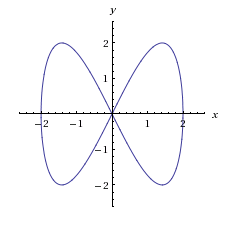
\includegraphics[width=0.55\textwidth]{task.png}
\end{figure}	
	
	
\textbf{Solution:}	
	
The curve gives us the assumption, that its symmetric about the x- and y-axis and about the origin. 

\begin{itemize}
	\item A graph will have symmetry about the x-axis if we get an equivalent equation when all the y’s are replaced with -y.
	\item A graph will have symmetry about the y-axis if we get an equivalent equation when all the x’s are replaced with -x.
	\item A graph will have symmetry about the origin if we get an equivalent equation when all the y’s are replaced with -y and all the x’s are replaced with -x.
\end{itemize}	
	
All of the above tests are true for $y^2 = 4x^2 - x^2$ which will make the computation of the area much simpler.\\

Let's also prove if the roots of -2 and 2 are right. To get y we have the function $y = \sqrt{x^2 \cdot (4-x^2)} \rightarrow y = \sqrt{x^2} \sqrt{4-x^2} \rightarrow y = x \sqrt{4-x^2}$\\

Test for 2: $2 \sqrt{4 - 2^2} = 0 \rightarrow 2 \cdot 0 = 0$\\
Test for -2: $2 \sqrt{4 - (-2)^2} = 0 \rightarrow 2 \cdot 0 = 0$\\

So, the roots are right. Which gives us the following integral


\begin{align*}
	2 \int_0^2 (x \sqrt{4-x^2}) \; dx
\end{align*}

Let $u = 4 - x^2$\\
$\frac{du}{dx} = -2x \rightarrow -2xdx = du$

\begin{align*}
	2 \cdot ( - \frac{1}{2} \int_0^2 \sqrt{u}\; du ) =\\ 
	2 \cdot ( -\frac{1}{2} \frac{2u^\frac{3}{2}}{3} \Bigg]_0^2 ) =\\
	- 2 \frac{u^\frac{3}{2}}{3} \Bigg]_0^2 = - 2 \frac{(4-x^2)^\frac{3}{2}}{3} \Bigg]_0^2 = \\
	(-2 ((4-2^2)^(3/2)/3)) - (-2 ((4-0^2)^(3/2)/3)) =
	\frac{16}{3}
\end{align*}

The area enclosed by this curve is $\frac{16}{3} \approx 5.33333$	
	
	
	
	
\item (\textbf{20 points}) Given the curve $y = 3x^\frac{3}{2}-1$.


\begin{enumerate}
	\item[(a)] Find the points on the curve at $x = 0$ and $x = 4$ and determine the length of the straight line between these points.\\
	\textbf{Solution:}	
	
	\item[(b)] Find the arc length of the curve from $x = 0$ to $x = 4$\\
	\textbf{Solution:}	
	
	
	
	\item[(c)] Compare the two results in (a) and (b) and try to explain your opinion.\\
	\textbf{Solution:}	
	
	
\end{enumerate}

	
	
\end{enumerate}

\end{document}
